% !TEX encoding = UTF-8
% !TEX TS-program = pdflatex
% !TEX root = ../tesi.tex

%**************************************************************
\chapter{Methodology}
\label{ch:methodology}
\intro{In this chapter we will present the datasets created and used for the visual odometry.}

- Introduction\\
- Research Design\\
- Research Questions and Hypotheses\\
- Setting and Sample\\
- Data Collection\\
- Data Analysis\\
- Conclusion\\


demonstration of fit between methods chosen and research question(s)
rationale for choosing materials, methods and procedures
details of materials, equipment and procedures that will allow others to:
replicate experiments
understand and implement technical solutions

%**************************************************************

\section{Defined goal}\label{sec:defined-goal}
%**************************************************************

Most recent adversarial attack methods described in \ref{subsec:taxonomy-textual-adversarial-attacks} successfully decrease the accuracy of the target model.
However, since the main goal of the research is to enhance the robustness of the target model, we need to ensure that the quality of the crafted adversarial examples should be high, because the target model will be re-trained with them.

A successful natural language adversarial example can be defined as a perturbation that fools the model and fulfils  a set of linguistic constraints.
As an example in sentiment analysis (Figure \ref{fig:3_adverarial_example}), an attacker can fool the system by changing only one word from “Perfect” to “Spotless,” which can completely change the predicted output without being discerned by humans.

\begin{figure}[h]
    \centering
    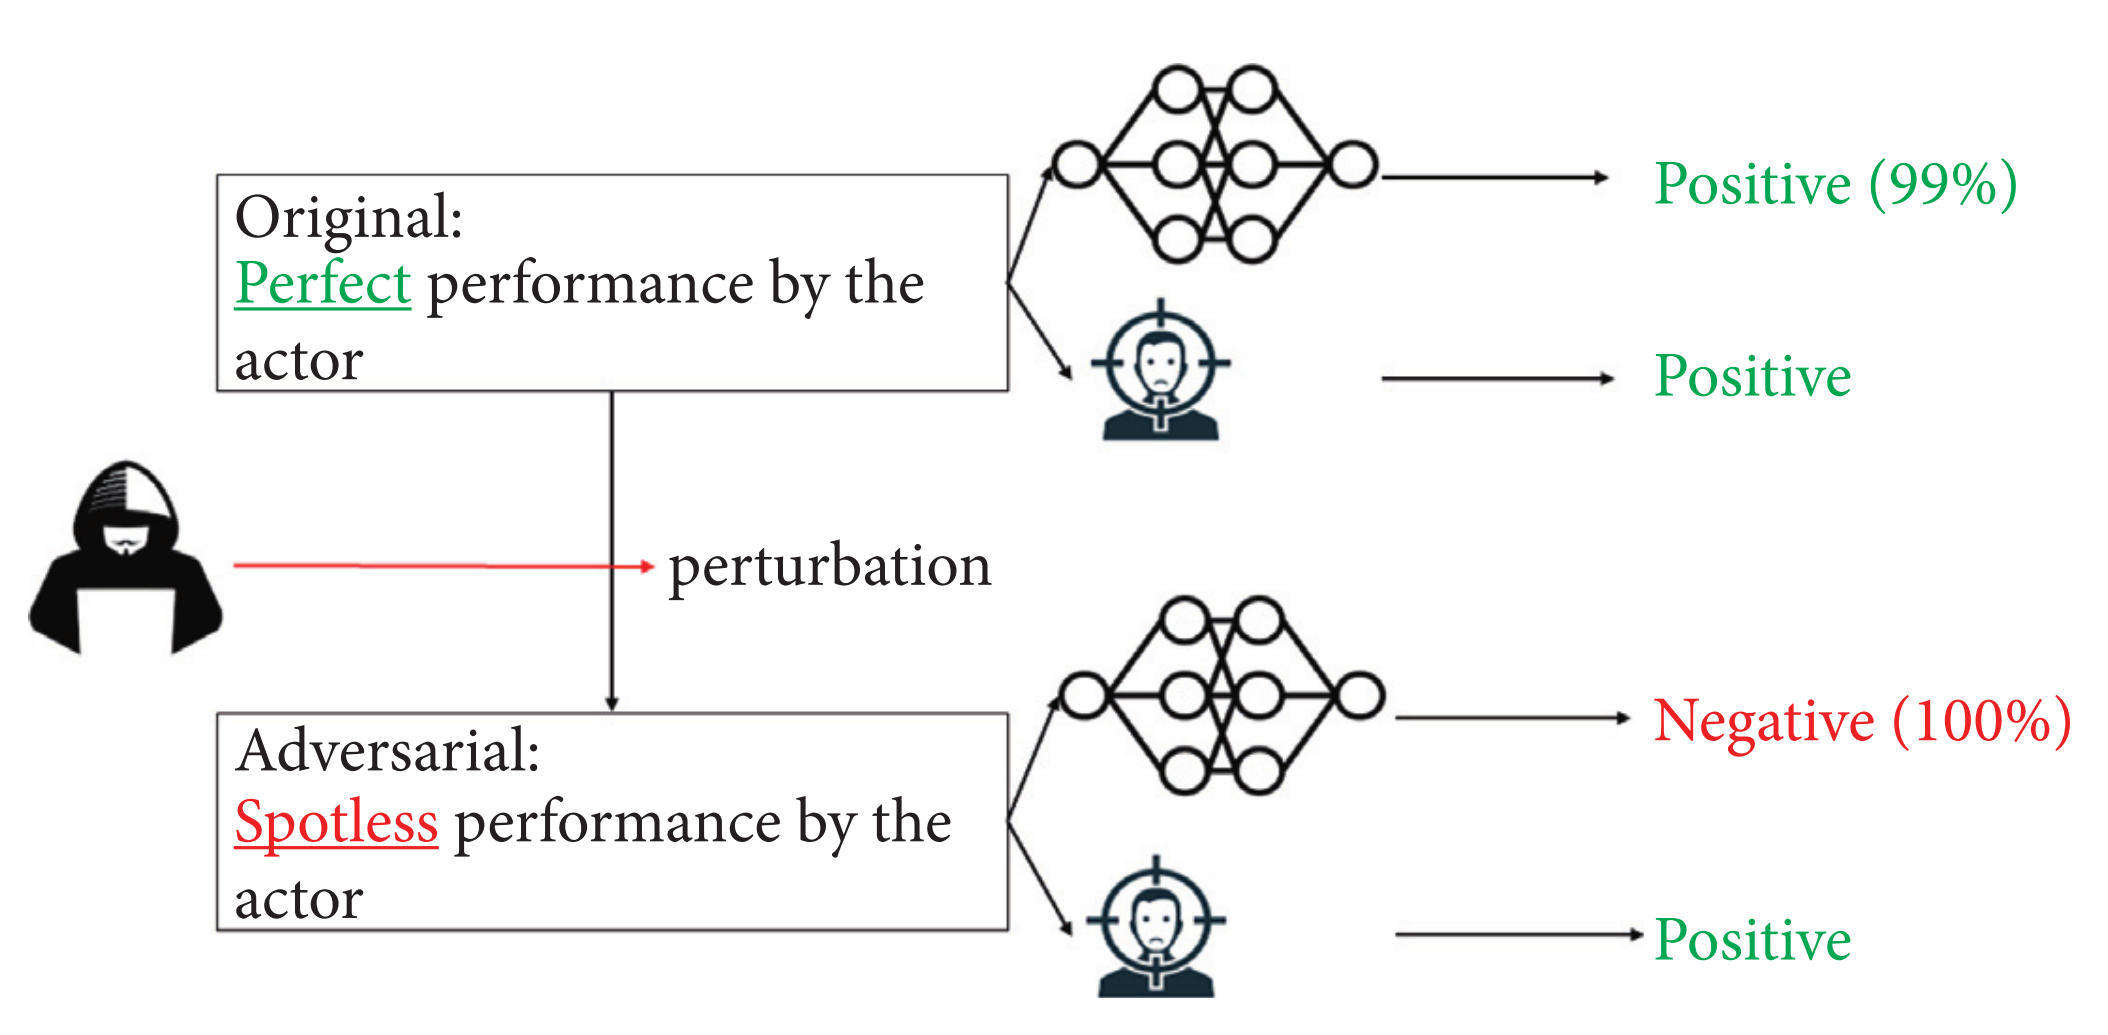
\includegraphics[width=0.7\linewidth]{images/3_adversarial_attack.png}
    \caption{Textual adversarial attack in sentiment analysis \cite{10.1155/2022/6458488}}
    \label{fig:3_adverarial_example}
\end{figure}

Formally, besides the ability to fool the target models, the outputs of a natural language attacking system should meet three key utility-preserving properties, defined by Jin et al. \cite{journals/corr/abs-1907-11932} as follows:
\begin{enumerate}
    \item \emph{human prediction consistency} - prediction by humans should remain unchanged;
    \item \emph{semantic similarity} -  the crafted example should bear the same meaning as the source, as judged by humans
    \item \emph{language fluency} - generated examples should look natural and grammatical
\end{enumerate}



%**************************************************************
\subsection{Problem to solve}\label{subsec:problem-to-solve}
Although attacks in NLP aspire to meet linguistic constraints, in practice, they frequently violate them.
Focusing on TextFooler and BERT-based attacks, they claim to create perturbations that preserve semantics, maintain grammaticality, and are not suspicious to readers. 
However, our inspection of the perturbations revealed that many violated these constraints.

On one hand, the perturbations generated by TextFooler solely account for the token level similarity via word embeddings, and not the overall sentence semantics. This can lead to out-of-context and unnaturally complex replacements.

On the other hand, with the capability of BERT, the perturbations crafted by BERT-based attacks are generated considering the context around. Therefore, the perturbations are fluent and reasonable.
Nevertheless, candidates generated from the masked language model can sometimes be antonyms or irrelevant to the original words, causing a semantic loss.

Table \ref{tab:3_1_wrong_adversarial_examples} highlights some examples of adversaries suffering from aforementioned issues.

\begin{table}[h]
    \footnotesize
    \centering
    \begin{tabularx}{\textwidth}{|l||l|X|}
      \hline
      Method & Label  & Samples \\
      \hline \hline
      TextFooler & Original (\textcolor{ForestGreen}{POS}) & generates an enormous feeling of empathy for its characters \\
                 & Perturbed (\textcolor{red}{NEG}) & leeds an enormous foreboding of empathy for its fonts
                 \\
      \hline
     
      BAE & Original (\textcolor{red}{NEG}) & bears is even worse than i imagined a movie ever could be.     \\
      & Perturbed (\textcolor{ForestGreen}{POS}) & bears is even greater than i imagined a movie ever could be.
    \\
        
      \hline
    \end{tabularx}
    \caption{Some adversarial samples generated with TextFooler and BAE}
  \label{tab:3_1_wrong_adversarial_examples}
\end{table}

%**************************************************************

\subsection{Research objective}\label{subsec:research-objective}

In order to address the research questions defined in Section \ref{sec:research-question}, 
we propose a new approach to generate adversarial examples that meet linguistic constraints.
In particular, we aim to demonstrate that:
\begin{itemize}
    \item using our evaluation framework defined in \ref{ch:experimental-results}, we can identify the weaknesses of existing attack methods;
    \item the utility-preserving properties measured on the proposed solution outperform the state-of-the-art;
\end{itemize}
 

%**************************************************************

%**************************************************************

\section{Research design}\label{sec:research-design}
%**************************************************************

Although adversarial attacks are a practical approach to evaluate robustness, most of them have the problem of being task-specific, not being well generalized.
Thus, this thesis is focused only on the text classification task, including sentiment analysis, topic classification, and natural language inference.

As baseline methods for adversarial attacks, we choose TextFooler \cite{journals/corr/abs-1907-11932} and BAE \cite{conf/emnlp/GargR20}.
Those are compared with the proposed method from a qualitative perspective. In addition, an efficiency assessment is carried out to measure the execution time.

\subsection{Attack category}\label{subsec:attack-category}

There are exploding combinations of the categories listed in Section \ref{subsec:taxonomy-textual-adversarial-attacks} into which our proposed attack method can fall into.
As a design choice, we defined the category of the attack in which we want to conduct our research.

Mainstream work has focused on word-level perturbation because of the large search space of substitution words and the hardness to maintain sentence semantics. 
Word-level methods usually maintain imperceptibility better than other attacks, so we also explored this category of attacks.

Differently from the baseline methods (TextFooler and BAE), our proposal attempt to generate adversarial examples in a white-box setting, which means that the attacker has access to the target model. 
This is a more realistic scenario, since the goal of the attacker is to craft adversaries with the purpose of enhancing the robustness of the target model. 
Thus, it has full access to the model and can exploit it to generate the perturbations.

The attack strategy and the adversarial goal are the same as the baselines, respectively importance-based and non-targeted attack.



%%**************************************************************

\section{Proposed solution}\label{sec:proposed-solution}
%**************************************************************

TextFooler and BERT-Attack suffer respectively from a lack of context and semantic similarity. 
We tried to combine their strengths in a novel method called SynBA (contextualized Synonym-Based adversarial Attack).
The main idea is to generate a set of synonyms for each word in the sentence, and then to select the best synonym for each word based on the context and semantic similarity.

%**************************************************************

\subsection{Intuition}\label{subsec:intuition}

In order to achieve semantic-consistent adversaries, we need to consider the cosine similarity between word embeddings or exploit a synonym dictionary.
While the synonyms retrieved from a thesaurus like WordNet are often somewhat related to the original word, the relation is often the wrong one for the given context.
Conversely, BERT has the potential to generate more fluent substitutions for an input text.

Our intuition is that the ranked list of candidates for word replacement is obtained from the so called \emph{SynBA score}, a weighted function summing up three scores:
\begin{itemize}
    \item \textbf{MLM score} - the confidence of candidate obtained by MLM (BERT)
    \item \textbf{Thesaurus score} - a score assigned to synonyms, hyponyms, and hypernyms of the original word in WordNet
    \item \textbf{Word embedding score} - the cosine similarity between the original word and the candidate
\end{itemize}

Combining these three scores, we can obtain a ranked list of candidates that results in a more contextualized and semantically consistent adversary.

%**************************************************************

\subsection{SynBA components}\label{subsec:synba-components}
SynBA has been implemented using TextAttack, a Python framework for implementing adversarial attacks in NLP (refer to section \ref{sec:text-attack} for more details).
Followig the framework structure, we decomposed our attack method into four components: a goal function, a set of constraints, a transformation, and a search method.

We reused some of the pre-existing components in TextAttack, such as the \texttt{UntargetedClassification} goal function, the \texttt{GreedyWordSwapWIR} search method and the constraints. 
The innovative part of SynBA is the \texttt{WordSwapMultimodal} transformation, implementing the SynBA score mechanism.
Table \ref{tab:3_3_comparing_components} summarizes the differences between SynBA and the two baselines.

\begin{table}[h]
    \footnotesize
\centering
\begin{tabular}{|c|c|c|c|}
\hline
\textbf{Components} & \textbf{TextFooler} & \textbf{BAE}  & \textbf{SynBA}\\ \hline
Search Method &  Deletion-based &   Deletion-based & Gradient-based\\ 
for Ranking Words & Word Importance & Word Importance & Word Importance \\ \hline
Transformation & Word Embedding & BERT MLM & SynBA score \\ \hline
 & POS  & POS & POS \\ 
 Constraints & USE & USE & Sentence-BERT \\ 
 & Word Embedding Distance &  & Word Embedding Distance \\ 
 &  &  & Max Modification Rate \\ \hline
 
\end{tabular}
\caption{Comparing SynBA components with TextFooler and BAE}
\label{tab:3_3_comparing_components}
\end{table}

%--------------------------------------------------------------
\subsubsection{Search Method}\label{subsubsec:search-method}

The search method is responsible for going through the search space of possible perturbations and  find a sequence of transformations that produce a successful adversarial example.

Greedy algorithms with word importance ranking are linear with respect to input length, with a complexity of $\mathcal{O}(W*T)$, where $W$ indicates the number of words in the input, $T$ is the maximum number of transformation options for a given input \cite{journals/corr/abs-2009-06368}. 

So in SynBA we use the \texttt{GreedyWordSwapWIR} search method, which is a greedy search method that iteratively applies the transformation to the input text, and selects the best candidate for each word based on the \acrfull{wir} score.
Words of the given input are ranked according to the importance function. Then, in order of descending importance, each word is substituted with the best candidate given by the transformation
that maximizes the scoring function until the goal is achieved, or all words have been perturbed.

The WIR is gradient-based, which means that it is able to rank the words in the input text exploiting the gradient of the loss function with respect to each token.

It is the same search method used by the attack component in A2T (see section \ref{subsec:a2t}).
Yoo et al. \cite{journals/corr/abs-2009-06368} showed that the gradient-ordering method is the fastest search method and provides competitive attack success rate when compared to the deletion-based method.
%--------------------------------------------------------------

\subsubsection{Transformation}\label{subsubsec:transformation}

To enforce semantic preservation, we designed the \texttt{WordSwapMultimodal} transformation function, which is not provided by TextAttack.
It computes a set of $k$ perturbations given a word in the input text selected by the search method, where $k$ is the number of candidates to be generated.

The transformation function is based on the SynBA score, which is described in Figure \ref{fig:3_3_synba_score}.
It is calculated for each word in the vocabulary and then they are ranked in descending order.
Tree components are used to compute the SynBA score: the \emph{MLM score}, the \emph{thesaurus score}, and the \emph{word embedding score}.

The \emph{MLM score} is the confidence of the candidate obtained by \texttt{bert-base-uncased}\footnote{\url{https://huggingface.co/bert-base-uncased}} MLM masking the word that we want to perturb.
Since the confidence is a probability value, we need to normalize it in order to have each component magnitude in the same range $[0,1]$.
So the vector output of the MLM is rescaled using a min-max scaling:
\begin{equation}
    x^\prime = \frac{x - \min(x)}{\max(x) - \min(x)}
\end{equation}

The \emph{thesaurus score} makes use of WordNet, a lexical database for the English language. Each word in the vocabulary is associated with a score depending on the relation with the original word:
\begin{itemize}
    \item \textbf{synonym} - the score is equal to 1
    \item \textbf{hyponym} - the score is equal to 0.5
    \item \textbf{hypernym} - the score is equal to 0.5
    \item \textbf{antonym} - the score is equal to -100 (to push the antonym out of the top $k$ candidates)
\end{itemize}
If the candidate is not in the WordNet \emph{synset}, the score is equal to 0.

The \emph{word embedding score} is the cosine similarity between the original word and the candidate. We used counter-fitting GloVe vectors \cite{conf/naacl/MrksicSTGRSVWY16} exploiting the property of antonym repeal and synonym attraction. 
This score falls already in the range $[0,1]$, so it does not need to be normalized.

It is likely that the vocalulary of the MLM is different from the one of WordNet and GloVe, so we consider the union of the three vocabularies.
Then the three scores are combined using a weighted sum, where the weights $\lambda_1, \lambda_2, \lambda_3$ are hyperparameters that can be tuned.

Reference words in the original text that are numbers, non-alphabetical, stop words or one-character words are not perturbed, since they could easily influence the meaning of the sentence (e.g. in a movie review, if we alter the number of stars from 5 to 1, the polarity of the review changes).
Meanwhile candidates that are subwords, punctuations or contain multiple words are discarded.

Before replacing each candidate to the reference word in the input text, we recover the original capitalization of the word, since the MLM and the word embedding models are case insensitive.

\begin{figure}
    \centering
    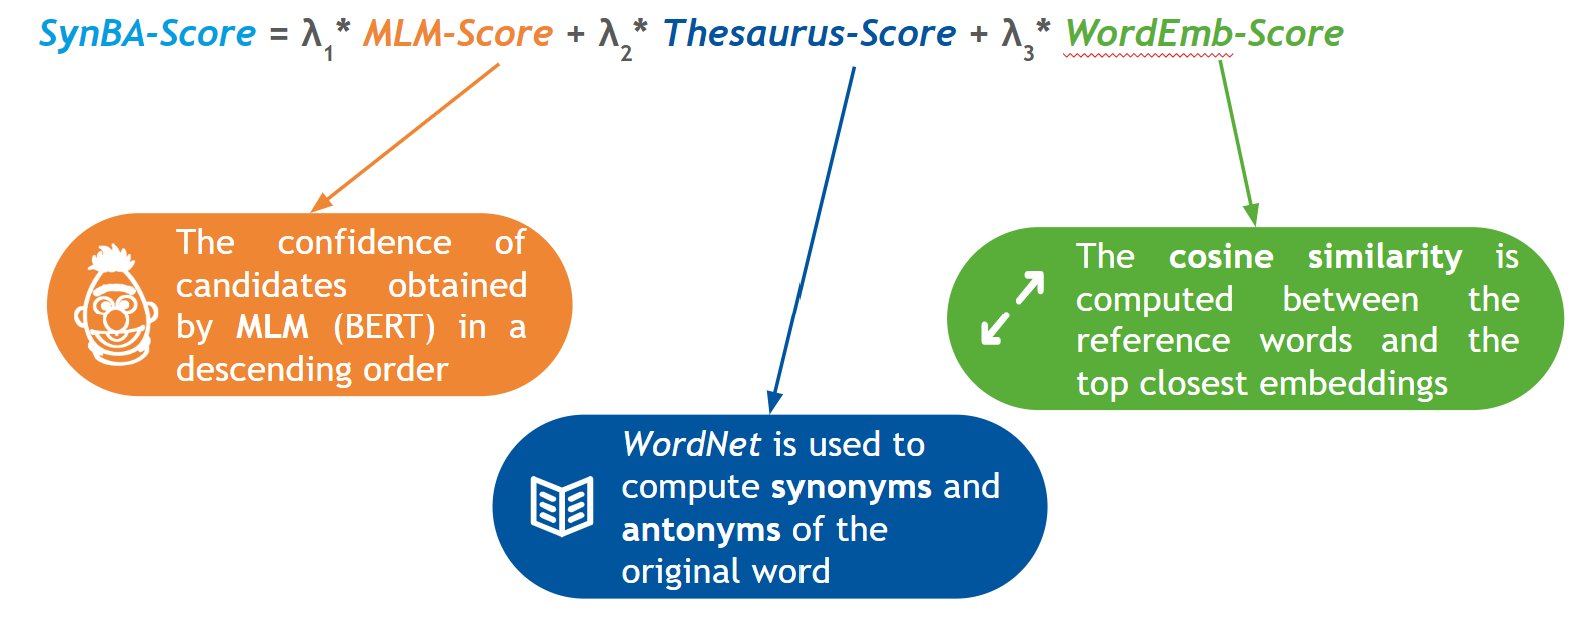
\includegraphics[width=0.8\linewidth]{images/3_3_synba_score.png}
    \caption{SynBA score}
    \label{fig:3_3_synba_score}
\end{figure}

%--------------------------------------------------------------

\subsubsection{Constraints}\label{subsubsec:constraints}

Constraints are used to avoid the generation of adversarial examples that are too different from the original input text.
Those perturbations that do not satisfy all constraints are discarded.

We reused the following constraints, which are already implemented in the framework:
\begin{itemize}
    \item \texttt{PartOfSpeech} - constraints perturbations to only swap words with the same part of speech. It uses the NLTK universal part-of-speech tagger;
    \item \texttt{WordEmbeddingDistance} - throws away perturbations for which the distance between the original word and the candidate is lower than a threshold $t=0.6$;
    \item \texttt{MaxModificationRate} - limits the number of words that can be perturbed in the input text to a maximum percentage $p=0.2\%$. Since text length can vary a lot between samples, and a $p$ modification limit might not make sense for very short text, it is guaranteed that at least 4 words can be perturbed;
    \item \texttt{BERT} - checks whether the \acrfull{sts} between the original and the perturbed text is higher than a threshold $t=0.7$. The  sentence embeddings are computed using a Sentence-BERT \cite{reimers2019sentencebert} pre-trained model. In particular, we used the \texttt{stsb-mpnet-base-v2}\footnote{\url{https://huggingface.co/sentence-transformers/stsb-mpnet-base-v2}} model, which is first trained on NLI data, then we fine-tuned them on the STS benchmark dataset. This generate sentence embeddings that are especially suitable to measure the semantic similarity between sentence pairs.
    It has an higher STSb performance score ($88.57$) compared to USE ($74.92$). This performance metric is the Spearman rank correlation $\rho$ between the cosine similarity of sentence representations and the gold labels for various STS tasks.
\end{itemize}           
%--------------------------------------------------------------

\subsubsection{Goal Function}\label{subsubsec:goal-function}

The goal function in SynBA is \texttt{UntargetedClassification}, which attempts to minimize the score of the correct label until it is no longer the predicted label.
Attack ends when the predicted label of the perturbed text is different from the original one.
Otherwise a transformation is performed on the next most important word, until all words are perturbed.

The goal function result status can be:
\begin{itemize}
    \item \texttt{Succeded} - the attack was successful and the predicted label is different from the original one;
    \item \texttt{Failed} - the attack method was not able to find a perturbation that fooled the model;
    \item \texttt{Skipped} - the ground truth label is different from the predicted one
\end{itemize}

%**************************************************************

\subsection{Hyperparameter Tuning}\label{subsec:hyperparameter-tuning}

In order to find the best hyperparameters for \emph{SynBA score}, 

%**************************************************************

\subsection{Candidates ranking calibration}\label{subsec:candidates-ranking-calibration}
The candidate pool range is the major hyperparameter used in the BERT-Attack algorithm. As seen in Figure 2, the attack rate is rising along with the candidate size increasing. Intuitively, a larger 
K would result in less semantic similarity. However, the semantic measure via Universal Sentence Encoder is maintained in a stable range, (experiments show that semantic similarities drop less than 2%), indicating that the candidates are all reasonable and semantically consistent with the original sentence. Further, a fixed candidate number could be rigid
in practical usage, so we run a test using a threshold to cut off candidates that are less possible as a plausible perturbation. As seen in Table 4, when using a flexible threshold to cut off unsuitable candidates, the attacking process has a lower query number. This indicates that some candidates predicted by the masked language model with a lower prediction score may not be meaningful so skipping these candidates can save the unnecessary queries.

\begin{figure}
    \centering
    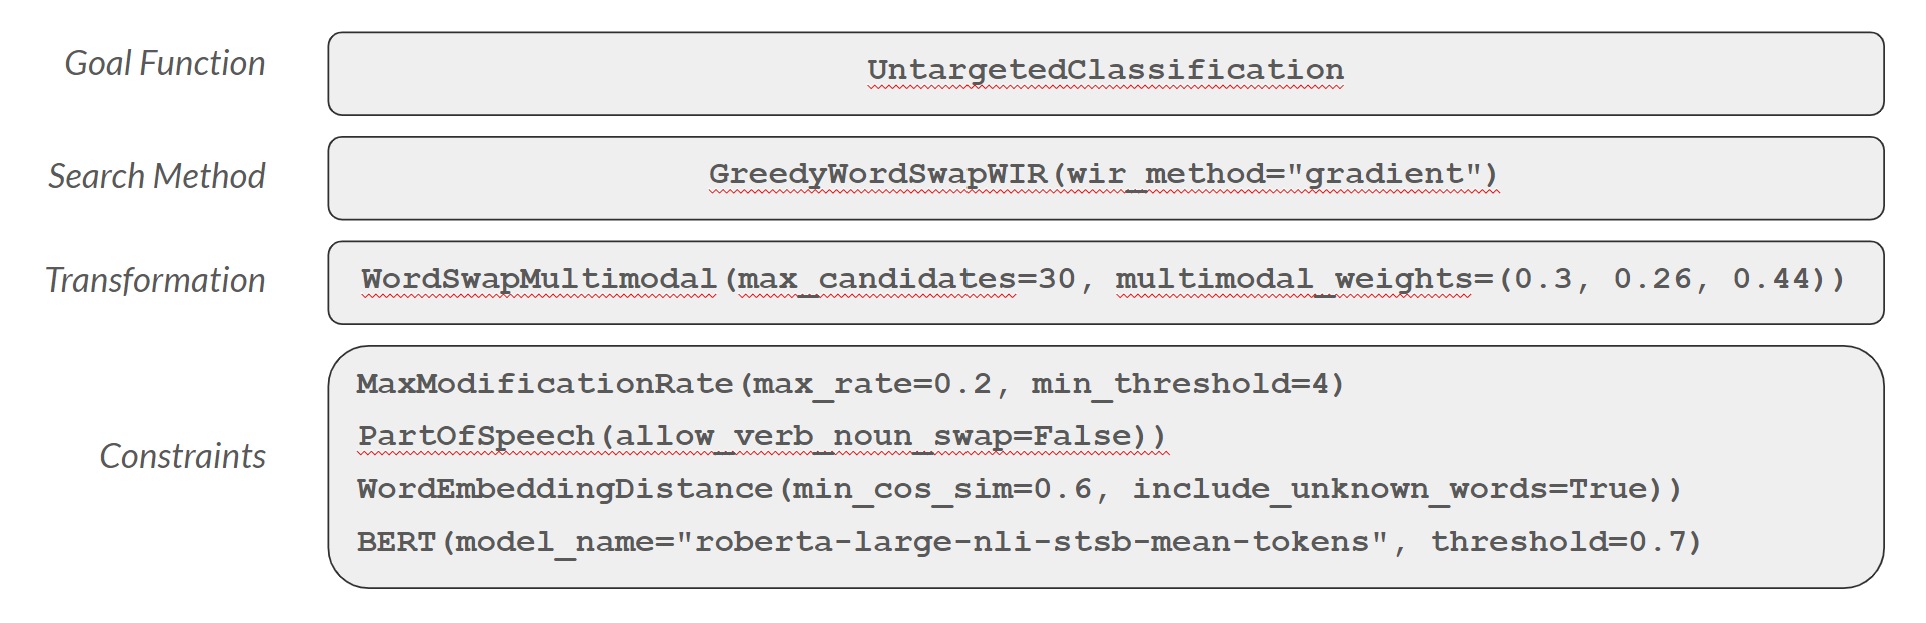
\includegraphics[width=0.8\linewidth]{images/3_synba_components.png}
    \caption{SynBA components on TextAttack framework}
    \label{fig:3_3_synba_components}
\end{figure}

%**************************************************************



%**************************************************************

\section{Evaluation metrics}\label{sec:evaluation-metrics}

Since our objective is to evaluate the quality of the adversarial examples crafted by SynBA, TextFooler and BAE, 
we need to define some sets of metrics that can be used to compare the effectiveness and efficiency of the different methods.

\subsection{Attack metrics}\label{subsec:attack-metrics}

The first set of metrics is used to evaluate the statistics of the attack process:
\begin{itemize}
    \item \textbf{Succeeded / Failed / Skipped}: number of input samples that are respectively successfully attacked, failed to be attacked, or skipped;
    \item \textbf{Original accuracy}: accuracy of the model on the original input samples;
    \item \textbf{Accuracy under attack}: accuracy of the model on the attacked input samples;
    \item \textbf{Attack success rate}: percentage of input samples that are successfully attacked;
    \item \textbf{Average perturbed word}: average percentage of words that are perturbed in the attacked input samples;
\end{itemize}
%**************************************************************

\subsection{Quality metrics}\label{subsec:quality-metrics}

The second set of metrics is used to evaluate the quality of the adversarial examples generated:
\begin{itemize}
    \item \textbf{Average SBERT similarity}: average semantic similarity between the original and the attacked input samples. It uses the same model of BERT constraint (\texttt{stsb-mpnet-base-v2}) to compute the sentence embeddings of the texts;
    \item \textbf{Average original perplexity}: average perplexity of the original input samples;
    \item \textbf{Average attacked perplexity}: average perplexity of the attacked input samples;
    \item \textbf{Attack contradiction rate}: percentage of adversarial examples that results in a contradiction between the original and the attacked input samples.
\end{itemize}

Fixing a good LM, perplexity can be used to measure the language fluency of a text. 
It is defined as the inverse probability of the text, so the lower the perplexity, the more fluent the text is.
We used a pre-trained small GPT-2 \cite{gpt2} model to compute the perplexity of input texts before and after the attack.

Instead, the contradiction rate makes use of an NLI model to assess whether the original input (premise) contradicts the adversarial example (hypothesis).
The idea is that if the perturbation introduces antonyms or changes the polarity of the sentence, a textual entailment model should be able to detect it. The lower the rate of contradiction, the better the attack method.
We used the pre-trained cross-encoder \texttt{nli-deberta-v3-base}\footnote{\url{https://huggingface.co/cross-encoder/nli-deberta-v3-base}}, which takes as input a text pair and outputs a probability distribution over the three classes: \emph{entailment}, \emph{contradiction}, and \emph{neutral}.
It is trained on the SNLI \cite{journals/corr/BowmanAPM15} and MultiNLI \cite{journals/corr/WilliamsNB17} datasets and achieves a high accuracy of 90.04\% on the MNLI mismatched set.
Only the pairs for which the contradiction output probability is the highest are considered contradictory.

%**************************************************************

\subsection{Efficiency metrics}\label{subsec:performance-metrics}

In order to evaluate the efficiency of the attack methods, we also define a set of metrics that can be used to compare the execution time of the different methods:
\begin{itemize}
    \item \textbf{Average attack time}: average time needed to craft an adversarial example;
    \item \textbf{Average WIR time}: average time needed to compute the word importance ranking;
    \item \textbf{Average transformation time}: average time needed to perform a transformation step;
    \item \textbf{Average constraints time}: average time needed to check the constraints;
    \item \textbf{Average query number}: average number of queries to the target model used to craft an adversarial example.
\end{itemize}

%**************************************************************

%**************************************************************